\documentclass[12]{article}
\usepackage{listings}
\usepackage{color}
\usepackage{tikz}
\usetikzlibrary{positioning,shapes,shadows,arrows}

\title{B Tag SF Procedure}
\author{Brett Jackson}

\begin{document}
\maketitle
\section{Introduction}
This is just a short document to document my understanding of how we compute our b-tag scale factors (SF).
We are using the SUSYTools BTagCalib tool ({\color{red}do we really want to use this tool?}) to compute our b-tag SF.
This tool takes as an input the following:

\begin{lstlisting}
m_b_tag_calibration->BTagCalibrationFunction( pt_list
                                            , eta_list
                                            , mv1_list
                                            , pdgid_list
                                            , is_sherpa
                                            );
\end{lstlisting}

\begin{itemize}
  \item pt\_list: \texttt{std::vector<float>} of the $p_T$ values of each of our jets
  \item eta\_list: \texttt{std::vector<float>} of the $\eta$ values of each of our jets
  \item mv1\_list: \texttt{std::vector<float>} of the MV1 values of each of our jets
  \item pdgid\_list: \texttt{std::vector<int>} of the flavor for each of our jets
  \item is\_sherpa: boolian to tell the tool if this is a Sherpa sample
\end{itemize}

It should be noted that all the jets which could possibly be tagged as a b-tagged jet are considered here, not just the jets that are flagged as b-tagged jets 

This function returns a pair of vectors. The first contains the following entries:
\begin{itemize}
\item 0 : standard
\item 1 : B-jet efficiency down
\item 2 : C-jet efficiency down
\item 3 : mistag rate efficiency down
\item 4 : B-jet efficiency up
\item 5 : C-jet efficiency up
\item 6 : mistag rate efficiency up
\end{itemize}
The second vector contains a list of the individual jet weights.

So, what happens when we call this function?

\section{Procedure}

The SUSYTools function appears to try and account for the difference in tagging efficiencies and mis-tagging rates (both light jets being mis-tagged as b-tagged jets, and b jets being mis-tagged as light flavor jets).
The pseudocode for this procedure is:

\begin{lstlisting}
sf = 1.
for j in jet_list:
    if isBTagged(j):
        sf *= getScaleFactor(j.pt, j.eta, j.flavor)
    else:
        sf *= getInefficiencyScaleFactor(j.pt, j.eta, j.flavor)
return sf
\end{lstlisting}

Essentially, this boils down to
\begin{equation}
  SF =
  \prod_{j \in \mathrm{\{b-tagged\}}} SF_j^{\mathrm{eff}}
  \prod_{j \in \mathrm{\{Not\, b-tagged\}}} SF_j^{\mathrm{ineff}}
\end{equation}

More stuff goes on in this function, but this appears to be the main idea.
To my understanding, this tool finds the difference in probability between data and MC of measureing a certain combination of tags and anti-tags given a set of jets.

\section{Example}
Suppose we have an event with four jets, two from b quarks, and two light flavor jets.
In this event, jet 1 and 3 are the (truth) b jets, and jets 2 and 4 are the light flavor jets.

\begin{center}
  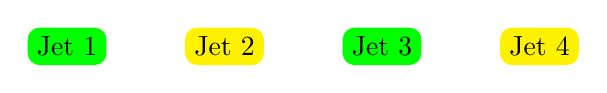
\begin{tikzpicture}
    \node[rectangle, rounded corners=1ex, fill=green , text=black] (j1) at (-3,0) {Jet 1};
    \node[rectangle, rounded corners=1ex, fill=yellow, text=black] (j2) at (-1,0) {Jet 2};
    \node[rectangle, rounded corners=1ex, fill=green , text=black] (j3) at (+1,0) {Jet 3};
    \node[rectangle, rounded corners=1ex, fill=yellow, text=black] (j4) at (+3,0) {Jet 4};
  \end{tikzpicture}
\end{center}

Of course, we would like to tag jets 1 and 3 as b-tagged jets and jets 2 and 4 as not-b-tagged jets.

\begin{center}
  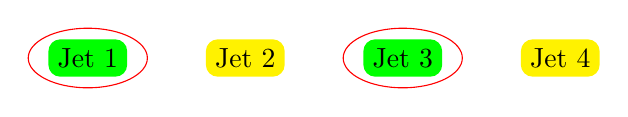
\begin{tikzpicture}
    \node[rectangle, rounded corners=1ex, fill=green , text=black] (j1) at (-3,0) {Jet 1};
    \node[rectangle, rounded corners=1ex, fill=yellow, text=black] (j2) at (-1,0) {Jet 2};
    \node[rectangle, rounded corners=1ex, fill=green , text=black] (j3) at (+1,0) {Jet 3};
    \node[rectangle, rounded corners=1ex, fill=yellow, text=black] (j4) at (+3,0) {Jet 4};

    \node[ellipse, minimum height = 5ex, minimum width = 10ex, draw, color=red] (b1) at (-3,0) {};
    \node[ellipse, minimum height = 5ex, minimum width = 10ex, draw, color=red] (b3) at (+1,0) {};
  \end{tikzpicture}
\end{center}

In this scenario, our SF will be given by

\begin{equation}
  SF =
  SF_{1}^{\mathrm{eff}}
  \cdot
  SF_{2}^{\mathrm{ineff}}
  \cdot
  SF_{3}^{\mathrm{eff}}
  \cdot
  SF_{4}^{\mathrm{ineff}}
\end{equation}

Alternatively, we could mis-tag jets 2 and three.

\begin{center}
  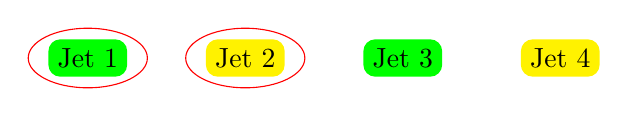
\begin{tikzpicture}
    \node[rectangle, rounded corners=1ex, fill=green , text=black] (j1) at (-3,0) {Jet 1};
    \node[rectangle, rounded corners=1ex, fill=yellow, text=black] (j2) at (-1,0) {Jet 2};
    \node[rectangle, rounded corners=1ex, fill=green , text=black] (j3) at (+1,0) {Jet 3};
    \node[rectangle, rounded corners=1ex, fill=yellow, text=black] (j4) at (+3,0) {Jet 4};

    \node[ellipse, minimum height = 5ex, minimum width = 10ex, draw, color=red] (b1) at (-3,0) {};
    \node[ellipse, minimum height = 5ex, minimum width = 10ex, draw, color=red] (b2) at (-1,0) {};
  \end{tikzpicture}
\end{center}

This would give us the following scale factor.
\begin{equation}
  SF =
  SF_{1}^{\mathrm{eff}}
  \cdot
  SF_{2}^{\mathrm{eff}}
  \cdot
  SF_{3}^{\mathrm{ineff}}
  \cdot
  SF_{4}^{\mathrm{ineff}}
\end{equation}

\section{Possible issues}

A possible issue I could see with this method is related to the fact that we allow for more than 2 b-tagged jets.
We only consider the leading two b-tagged jets in our event, so in the above scenario, the two scenarios are equivalent for our purposes:

\begin{center}
  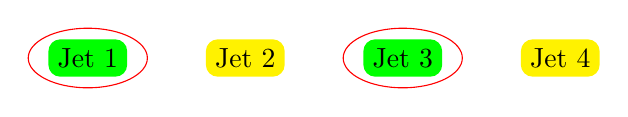
\begin{tikzpicture}
    \node[rectangle, rounded corners=1ex, fill=green , text=black] (j1) at (-3,0) {Jet 1};
    \node[rectangle, rounded corners=1ex, fill=yellow, text=black] (j2) at (-1,0) {Jet 2};
    \node[rectangle, rounded corners=1ex, fill=green , text=black] (j3) at (+1,0) {Jet 3};
    \node[rectangle, rounded corners=1ex, fill=yellow, text=black] (j4) at (+3,0) {Jet 4};

    \node[ellipse, minimum height = 5ex, minimum width = 10ex, draw, color=red] (b1) at (-3,0) {};
    \node[ellipse, minimum height = 5ex, minimum width = 10ex, draw, color=red] (b3) at (+1,0) {};
  \end{tikzpicture}
\end{center}
\begin{equation}
  SF =
  SF_{1}^{\mathrm{eff}}
  \cdot
  SF_{2}^{\mathrm{ineff}}
  \cdot
  SF_{3}^{\mathrm{eff}}
  \cdot
  SF_{4}^{\mathrm{ineff}}
\end{equation}

\begin{center}
  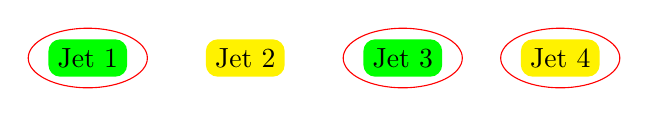
\begin{tikzpicture}
    \node[rectangle, rounded corners=1ex, fill=green , text=black] (j1) at (-3,0) {Jet 1};
    \node[rectangle, rounded corners=1ex, fill=yellow, text=black] (j2) at (-1,0) {Jet 2};
    \node[rectangle, rounded corners=1ex, fill=green , text=black] (j3) at (+1,0) {Jet 3};
    \node[rectangle, rounded corners=1ex, fill=yellow, text=black] (j4) at (+3,0) {Jet 4};

    \node[ellipse, minimum height = 5ex, minimum width = 10ex, draw, color=red] (b1) at (-3,0) {};
    \node[ellipse, minimum height = 5ex, minimum width = 10ex, draw, color=red] (b3) at (+1,0) {};
    \node[ellipse, minimum height = 5ex, minimum width = 10ex, draw, color=red] (b4) at (+3,0) {};
  \end{tikzpicture}
\end{center}
\begin{equation}
  SF =
  SF_{1}^{\mathrm{eff}}
  \cdot
  SF_{2}^{\mathrm{ineff}}
  \cdot
  SF_{3}^{\mathrm{eff}}
  \cdot
  SF_{4}^{\mathrm{eff}}
\end{equation}

These two scenarios would give different scale factors based on the jet that we don't consider since it's the third b-tagged jet.
Is this what we want? I'm going to look into what the top group does for their measurements.

\end{document}
